\documentclass{sig-alternate}
\usepackage[numbers, sort, compress]{natbib}
\usepackage{graphics}
\usepackage{graphicx}
\usepackage{epstopdf}
\usepackage{color}
\usepackage{hyperref}
\usepackage{pdfsync}
\usepackage{mdwlist}


\begin{document}

\conferenceinfo{XSEDE '12, July 16-20, 2012, Chicago, USA.} {}
\CopyrightYear{2012}
\crdata{}
%\clubpenalty=10000
%\widowpenalty = 10000

% \title{BigJob: Lessons of Supporting High Throughput High Performance
%   Ensembles on XSEDE}

\title{The Anatomy of a succesful ECSS Project: Leveraging Expertise
  of Users, Software-providers and XSEDE Personnel}

\numberofauthors{2}
\author{
\alignauthor Yaakoub El Khamra\\
       \affaddr{A Shady Computing Center}\\
       \affaddr{Austin, TX} \\
       \email{}
\alignauthor Melissa Romanus\\
       \affaddr{XXXXXX}\\
       \affaddr{XXXX} \\
       \email{}
% \alignauthor Pradeep Mantha\\
%        \affaddr{Center for Computation and Technology}\\
%        \affaddr{Louisiana State University}\\
%        \affaddr{216 Johnston}\\
%        \affaddr{Baton Rouge, LA}\\
%        \email{pmantha@...}
% \alignauthor Matt McKenzie\\
%        \affaddr{}\\
%        \email{pmantha@...}
}

\maketitle


\begin{abstract}
\end{abstract}


\newif\ifdraft 
\drafttrue 
\ifdraft
\newcommand{\mrnote}[1]{{\textcolor{green} { ***MR: #1 }}}
\newcommand{\jhanote}[1]{ {\textcolor{red} { ***SJ: #1 }}}
\newcommand{\yyenote}[1]{ {\textcolor{cyan} { ***YYE: #1 }}}
\newcommand{\pmnote}[1]{ {\textcolor{blue} { ***PM: #1 }}}
\newcommand{\todo}[1]{ {\textcolor{red} { ***TODO: #1 }}}
\newcommand{\fix}[1]{ {\textcolor{red} { ***FIX: #1 }}}
\newcommand{\reviewer}[1]{} \else \newcommand{\yyenote}[1]{}
\newcommand{\mrmnote}[1]{} \newcommand{\pmnote}[1]{}
\newcommand{\jhanote}[1]{} \newcommand{\todo}[1]{ {\textcolor{red} {
      ***TODO: #1 }}} \newcommand{\fix}[1]{} \fi



\category{D.1.3}{Software}{Concurrent Programming}{ Distributed programming/parallel programming} 
\category{J.3}{Computer Applications}{Bioinformatics}

\section*{General Terms}{Design,Measurement,Theory}

 \keywords{}

\section{INTRODUCTION}

\subsection{ECSS: Extended Collaborative Support Service }

\section{Background}

\subsection{SAGA: Simple API for Grid Applications}

\subsection{BigJob: SAGA Pilot-Job Implementation}

\subsection{Scientifc Applications of SAGA / BigJob}

\subsection{ECSS Projects}

\mrnote{brief outline and science objectives of two projects,
  including Charles Laughton, Tom Bishop, Rutgers chemists}

\section{SAGA and BigJob on XSEDE}
\mrnote{SW description of SAGA, SW description of BigJob}

\section{CSA Deployment on XSEDE Machines}

%\begin{table}
%\begin{tabular}{| c | c | c |}
%\hline
%Machine & Adaptors Supported & \\ \hline
%Lonestar & & \\ \hline
%Ranger & & \\ \hline
%Kraken & & \\ \hline
%Trestles & & \\ \hline
%\end{tabular}
%\caption{CSA Deployments on XSEDE Resources}
%\label{table:CSA-Deployments}
%\end{table}

\subsection{Developments and Setbacks}
\mrnote{List initial setbacks, Show how the setbacks created new
  developments. (Pradeep's new adaptors)}

\subsection{Testing and Documentation Process}
\mrnote{Show how it is a team effort, BigJob deployment pipeline,
  Interaction with chemists to address their issues and formulate
  scripts to accomodate their needs}

\section{Initial Results} \mrnote{Show work from chemists (if
  available), Applicability of BigJob to other applications beyond RE
  / chemists}

\section{Conclusions and Future Work}
\mrnote{Further deployments, Replica exchange? File staging?,
  Continued support for chemists, Do we want to get into pilot job
  stuff?}


% \begin{figure}
%  \centering
% 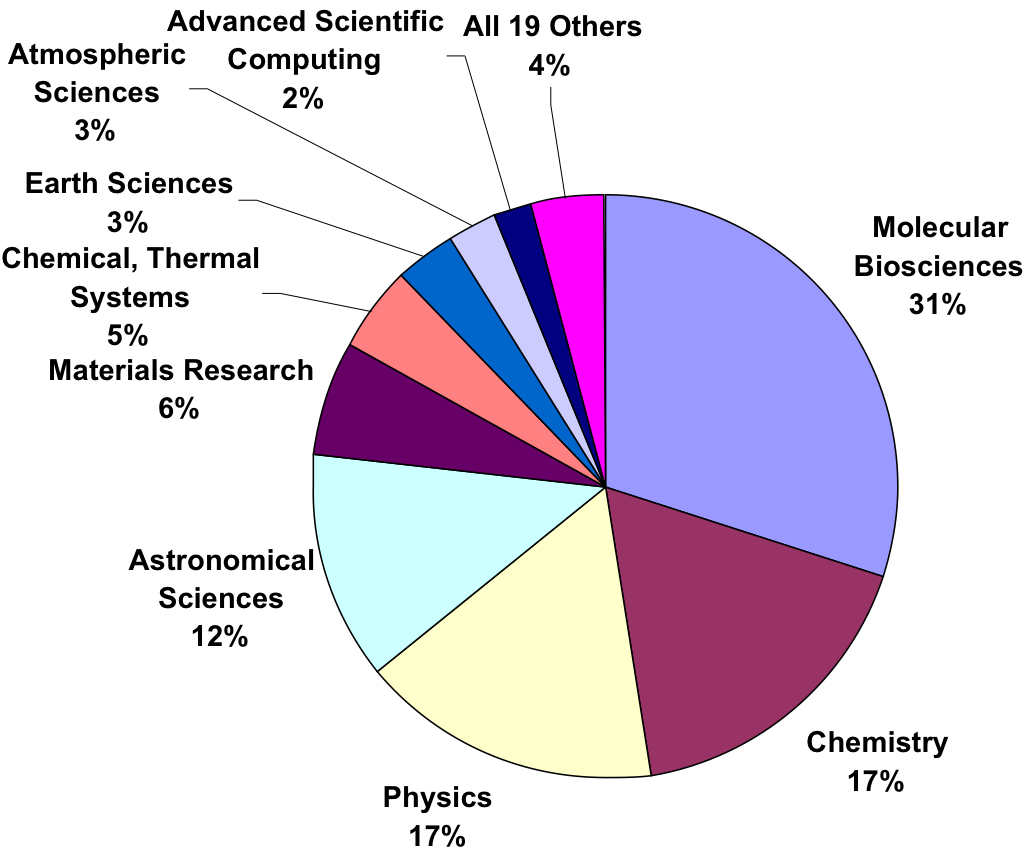
\includegraphics[scale=0.40]{figures/teragrid-discipline07}
% \caption{\small 2007 Usage statistics for the TeraGrid.  (Reference
%   \url{http://www.teragridforum.org/mediawiki/images/9/90/II_WorkShop_G-HPC_Nework_2009-Towns.pdf})}
%   \label{tg2007}
% \end{figure}


\section{Acknowledgments}
We are grateful to Andre Luckow and Ole Weidner for their work for
SAGA and SAGA-BigJob development.  Computing resources used for this
work were made possible via NSF TRAC award TG-MCB090174 and LONI
resources.  This document was developed with support from the National
Science Foundation (NSF) under Grant No.  0910812 to Indiana
University for ``FutureGrid: An Experimental, High-Performance Grid
Test-bed.''.

\bibliographystyle{abbrv}
\bibliography{tg11}
\end{document}

